\documentclass[12pt]{article}
\usepackage{ctex}
\usepackage{amsmath}
\usepackage{graphicx}
\usepackage{longtable}
\usepackage{booktabs}
\usepackage{geometry}
\usepackage{CJK}
\usepackage{float}
\usepackage{titling}
\usepackage{fancyhdr}
\usepackage{setspace}
\usepackage{hyperref}
\usepackage{listings}
\usepackage{xcolor}


\hypersetup{
	pdfborder={0 0 0},  % 关闭边框
}
\geometry{a4paper}

\title{ \textbf{基于多种统计分析方法的房租价格影响因素研究及定价策略建议}}
\date{}
\pagestyle{fancy}
\fancyhead[L]{}
\fancyhead[C]{2025年北京理工大学数学建模竞赛} 
\fancyhead[R]{}
\renewcommand{\abstractname}{\Large 摘要} 



\begin{document}
\begin{CJK}{UTF8}{gbsn}
	
	\thispagestyle{fancy}
	
	
\setlength{\droptitle}{-3cm}
	\thispagestyle{fancy}
	\maketitle  % 生成标题页
	
	\setcounter{page}{1}
	
	\vspace{-7em}
	\begin{abstract}  % 摘要环境
		\vspace{1em}
		Airbnb作为全球领先的短租平台,其房源价格的波动受多种因素的影响。合理的定价策略不仅直接影响房东的收入,还对房源的入住率和市场竞争力产生重要作用。本研究以Airbnb平台的房源价格为研究对象,结合\textbf{灰色关联分析}和\textbf{层析分析模型},对影响价格的主要因素进行了深入分析。通过收集2024年间纽约地区的Airbnb房源数据,重点研究了地理位置、房源类型等多种因素对房源价格的影响,并进一步探讨了如何制定最优的定价策略,以提高房东的收益并增强市场竞争力。
		
		\textbf{针对问题一},我们首先利用\textbf{KNN最临近插值法}来进行数据的缺失值补充,然后\textbf{箱线图}法发掘异常数据并处理,同时通过\textbf{饼状图}进行数据可视化进行数据初步分析,结果表明中低价位房源占比较高而高价位房源占比较低,即数据整体呈现\textbf{右偏性};同时人们更倾向于选择\textbf{发达地区与高私密性房源}进行居住。
		
		\textbf{针对问题二},我们对市场的\textbf{地理、房源类型、价格区间、房东规模}四个维度进行了细致的\textbf{描述性统计分析}与\textbf{散点图}可视化,获得了他们各自的特征与潜在价值。针对地理因素,我们发现了曼哈顿市场相较于其他市场的\textbf{高需求和高竞争性};针对房源类型,我们发现人们偏向于\textbf{私人房间},酒店房和共享房需要\textbf{优化定价}以提高入住率;针对价格因素,我们再次证实了\textbf{廉价}对于入住率的显著提高;针对房东拥有的住房规模,我们发现个人房东具有较强的\textbf{市场需求}而专业房东则更多\textbf{面向高端市场}。
		
		\textbf{针对问题三},我们通过\textbf{灰色关联度分析}获得了地理位置及房源对入住率和定价的影响。结果发现,\textbf{纽约的大区}对定价和入住率影响均最大,而\textbf{街区}则影响较小;\textbf{房间类型}对定价和入住率影响较小。我们得出了\textbf{地理位置是否优越}是影响定价和入住率的主要因素这一结论。
		
		\textbf{针对问题四},我们通过\textbf{层次分析法(AHP)}量化收益与入住率的权衡关系,并结合细分市场(房型、区域)的差异性,分层次构建判断矩阵,最终得出差异化定价策略。我们得出\textbf{曼哈顿整套房源}应选择\textbf{高价策略};\textbf{布鲁克林共享房间}应选择\textbf{低价策略}而\textbf{皇后区私人房间}则最好选择\textbf{平衡策略}的最终策略建议。\\
		
		\noindent\textbf{关键词:} KNN最临近差值法 ; 灰度关联分析法 ; 层次分析法 ; 房租定价策略
		
		
	\end{abstract}
	
	\newpage
	
	\section{问题背景}
	随着共享经济的蓬勃发展,短租平台已成为城市住宿市场的重要组成部分。作为全球领先的短租服务提供商,Airbnb的定价策略受到多维因素的复杂影响,包括房源的地理区位属性、设施配置特征、市场供需动态以及房东运营偏好等。科学合理的定价机制不仅关乎房东的经济收益与房源竞争力,还能让用户更愿意长期选择该平台,从而保障整个短租市场的良性运转。
	
	纽约市作为全球最具代表性的都市经济体,其短租市场具有高度异质性和动态性。然而,现有研究对多源异构数据的整合分析仍存在不足,尤其在细分市场特征挖掘、空间异质性对价格的影响机制以及收益与入住率的协同优化策略方面缺乏系统性探索。本研究基于2024年纽约市Airbnb房源数据,旨在通过数据驱动建模方法揭示市场运行规律,为房东与平台的精细化运营提供决策支持,亦可为城市共享经济监管政策的制定提供科学依据,助力实现短租市场的可持续发展。
	
	\begin{figure}[H]
		\centering
		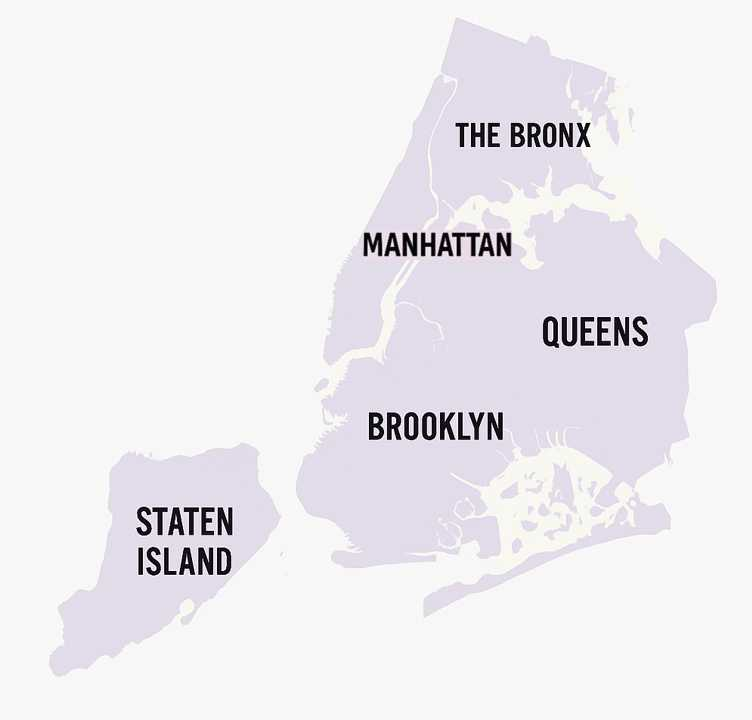
\includegraphics[width=0.7\textwidth]{pic/img.jpg} % 使用相对路径
		\caption{纽约房租定价策略}
		\label{fig:sample}
	\end{figure}
	
	\section{问题一的分析与求解}
	\subsection{问题一的分析}
	为便于后续开展描述性统计分析并准确探究各相关因素间的关联程度,需首先完成数据清洗与处理工作。该过程主要包括缺失值检测与处理、异常值处理以及重复数据处理三个关键步骤。
	
	在缺失值检测环节,发现\texttt{price}、\texttt{last\_review}和\texttt{license}三列存在缺失情况,其中\texttt{price}列缺失比例达39.2\%,且该变量与后续分析密切相关;而\\\texttt{last\_review}和\texttt{license}两列数据因其特性本身可能存在合理缺失,故无需进行填补处理。为确保数据完整性且不破坏原始分布规律及各变量间的关联特征,需通过计算与其他房源在其他特征维度上的相似性,采用相似房源价格进行插值填补。
	
	异常值处理主要针对\texttt{price}变量中存在的极端高值与极端低值。为降低极端值对后续统计分析的影响同时保持数据原有分布特征,采用极端值检测与替换方法,将超出合理区间的数值替换为修正区间的边界值,并辅以标识变量加以区分。相较于直接删除,该方法能更好地保持数据完整性以供后续分析使用。
	
	重复数据处理则基于房源ID和名称等唯一标识符进行检测与删除。
	
	完成数据清洗后,可进行描述性统计分析以定量呈现各指标的分布特征和基本统计规律。鉴于研究目标为提出兼顾收益与入住率的最优定价策略,并考虑不同细分市场和区域差异,统计分析应聚焦价格与入住率的分布特征,同时结合房源位置、类型等其他因素。
	
	基本统计量包括均值、中位数、众数、标准差、极差、四分位距、偏度与峰度等,其中前三者反映数据集中趋势,后五者刻画数据离散程度和分布形态。此外,可通过绘制频数分布直方图、核密度估计图及累积分布函数图等可视化手段直观展示数据分布特征。
	
	为支持后续定价策略分析,基于原始数据构建两个新变量:入住率\\(\texttt{occupancy})与年收入(\texttt{Annual\_Income}),其计算公式分别为:
	
	\begin{equation}
		\text{occupancy} = \frac{\text{availability\_365} - \text{vacancy\_days}}{\text{availability\_365}}
	\end{equation}
	
	
	\begin{equation}
	\text{Annual\_Income} = \text{price} \times (365 - \text{availability\_365})
	\end{equation}
	
	一般而言,房租价格分布呈现右偏特征,即中低价位房源占比较高而高价位房源占比较低,且部分高价房源会显著拉长分布尾端。可通过正态性检验验证该特征,并对价格变量进行对数变换以改善其正态性。同时,考虑到实际租赁市场中短期(约一个月)和长期(接近或超过一年)租客较多而中期租客较少的特点,入住率可能呈现双峰分布。可通过频数分布直方图对此现象进行验证。
	
	在正式进行建模分析前,我们先观察如下两张饼状图进行初步分析。
	
	\begin{figure}[H]
		\centering
		% 上方两张图片
		\begin{minipage}[b]{0.45\textwidth}
			\centering
			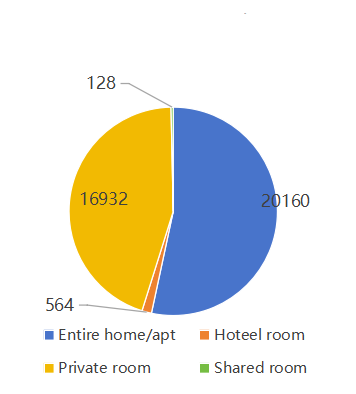
\includegraphics[width=\linewidth]{pic/11.png}
			\caption{不同房源类型饼状图}
		\end{minipage}
		\hfill
		\begin{minipage}[b]{0.45\textwidth}
			\centering
			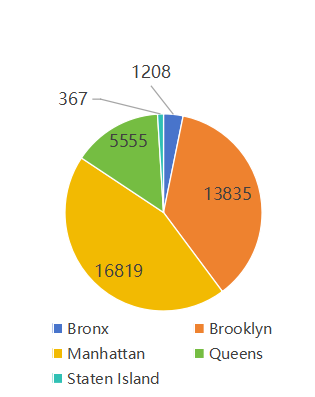
\includegraphics[width=\linewidth]{pic/12.png}
			\caption{不同区域饼状图}
		\end{minipage}
		
	\end{figure}
	
	房源类型分析:在Airbnb平台上,整套房源(Entire home/apt)占据了69.9\%的市场份额,表明大多数住客偏好具有私密性和独立空间的住宿选择,尤其适合家庭和长期居住的客群。私人房间(Private room)占28.4\%,由于其价格相对较低,吸引了预算有限的单人旅客或小团体入住。酒店房间(Hotel room)和共享房间(Shared room)的市场份额较小,分别为0.4\%和1.7\%。这些类型的房源需求相对较低,住客更倾向于选择具有更高私密性的住宿选项。
	地区分布分析:从市场区域的分布来看,布鲁克林(Brooklyn)和曼哈顿(Manhattan)在Airbnb市场中占据主导地位,分别占50.3\%和33.8\%的市场份额,这反映了这两个区域强劲的市场需求。布鲁克林在年轻人和创意行业群体中颇受欢迎,而曼哈顿作为经济和旅游的中心,吸引了大量的国际游客和商务人士。相比之下,皇后区(Queens)、斯坦顿岛(Staten Island)和布朗克斯(Bronx)则占据较小的市场份额,分别为7.7\%、4.5\%和1.4\%。这些区域的市场份额较小,可能与其地理位置、交通便利性以及整体旅游吸引力相关。
	
	\subsection{问题一的模型假设}
	本研究基于以下核心假设构建数据处理与分析框架:
	
	针对数据清洗处理,基于现实情况与相关经验,做出以下三个假设:
	
	\begin{itemize}
		\item 假设房源价格与地理位置(\texttt{neighbourhood\_group}、\texttt{latitude}、\texttt{longitude})及房源类型(\texttt{room\_type})存在显著关联性,且特征空间中邻近样本的价格具有相似性;
		\item 假设分类变量(\texttt{neighbourhood\_group}、\texttt{room\_type})经序数编码后仍能有效表征其属性差异,使用欧氏距离度量可准确反映样本间多维特征相似度;
		\item 假设在使用K临近插值法时,根据交叉验证所得最优K值能够平衡模型偏差与方差,确保插值结果既保留局部特征又不失稳健性。
	\end{itemize}
	
	这样以来,可以根据K临近插值法(KNN)进行缺失数据的填补。
	
	此外,默认缺失值机制为随机缺失(MAR),数据清洗过程不会引入系统性偏差,处理后的数据集可准确反映市场真实分布规律。
	
	针对价格分布特性,假设原始数据右偏态可通过自然对数变换改善其正态性,且箱线图法识别的异常值边界(19.5841美元)能有效区分正常经营价格与极端异常值。
	
	\subsection{问题一的模型构建与求解}
	\subsubsection{K近邻算法(KNN)的理论基础与实现}
	K近邻算法是一种基于距离度量的非参数化监督学习方法,其核心假设是特征空间中相似的样本具有相近的目标变量值。在缺失值填补问题中,KNN通过计算样本间的距离,识别出K个最近邻样本,并基于这些近邻的已知值进行缺失值估计。
	
	KNN算法的步骤如下:
	
	\begin{enumerate}
		\item \textbf{数据准备}  
		经检测,\texttt{price}列共有14,815个缺失值,填充前数据中的非缺失值数量为22,969,填充后数据总数应为37,784。缺失值占总样本量的39.2\%,占比显著。考虑到房源价格与地理位置和房源类型等特征存在复杂关联性,本研究采用K近邻(KNN)算法,基于数据集的\texttt{neighbourhood\_group}、\\\texttt{latitude}、\texttt{longitude}与\texttt{room\_type}特征对\texttt{price}列进行缺失值填补。其中,\texttt{neighbourhood\_group}、\texttt{latitude}与\texttt{longitude}反映房源的地理位置属性,\texttt{room\_type}反映房源类型属性。核心思路是通过特征空间中的相似性度量,找到与缺失样本最接近的K个近邻,利用其价格值的加权平均或简单平均进行填补。
		
		本研究在模型构建中着重处理分类变量的数值化转换与特征空间定义问题。针对\texttt{neighbourhood\_group}与\texttt{room\_type}两类分类特征,采用首字母序数编码法将其映射为离散整数值,确保相同类别房源在特征空间中距离趋近。具体而言,将\texttt{neighbourhood\_group}按首字母顺序依次赋值为1,2,\dots,\texttt{room\_type}同理处理,以此强化分类属性对距离计算的影响权重。在特征空间构建上,将编码后的分类变量与连续型地理坐标(\texttt{latitude}、\texttt{longitude})共同构成四维混合特征向量,采用欧氏距离度量样本相似性,其计算过程突出分类变量的主导作用——相同行政区域与房源类型的房源间距离显著小于仅地理坐标相近的样本。
		
		该设计有效捕捉纽约市租房市场中行政区域划分带来的系统性价格差异(如曼哈顿与其他区域的基准价差)及房源类型固有的定价层级特性(如整套房源与共享房间的价差结构),确保K近邻插值时优先选择具有相同市场属性的相似房源,最终实现价格缺失值的合理填补。
		
		\item \textbf{计算公式的模型构建}  
		本次计算中使用欧几里得距离度量公式,公式如下:
		
		\begin{equation}
			d(x, y) = \sqrt{\sum_{i=1}^{n} (x_i - y_i)^2}
		\end{equation}
		
		其中:\( x \) 和 \( y \) 是两个样本点,\( n \) 是特征维度,\( x_i \) 和 \( y_i \) 是两个样本在第 \( i \) 个特征上的值。
		
		通过简单平均法预测目标变量,公式如下:
		
		\begin{equation}
			\hat{y} = \frac{1}{K} \sum_{i=1}^{K} y_i
		\end{equation}
		
		其中:\( \hat{y} \) 为预测的目标变量值,\( K \) 为近邻数量,第 \( i \) 个近邻的目标值为 \( y_i \)(如房价、分类标签等)。
		
		计算均方误差(MSE)的公式如下:
		
		\begin{equation}
			MSE = \frac{1}{n} \sum_{i=1}^{n} (y_i - \hat{y}_i)^2
		\end{equation}
		
		当计算所得的 \( MSE \) 越小时,模型预测就越准确。
		
		通过对多次验证结果的均方误差取平均值获取交叉验证误差:
		
		\begin{equation}
			CV_{error} = \frac{1}{k} \sum_{i=1}^{k} MSE_i
		\end{equation}
		
		其中:
		- \( MSE_i \) 为第 \( i \) 折交叉验证的均方误差(使用 \( i \) 时),
		- \( k \) 为交叉验证的折数。
		
		本研究通过K折交叉验证确定KNN算法的最优近邻数K值。设定候选K值范围为1至15,采用5折交叉验证策略评估各K值的预测性能:将数据集随机划分为5个互斥子集,依次选取每个子集作为验证集,其余4个子集作为训练集,遍历所有候选K值。对于每个K值,基于欧氏距离计算验证集样本的K个最近邻,通过简单平均法预测目标变量(房价),并计算均方误差(\( MSE \))衡量预测精度,其中 \( n \) 为验证集样本数,\( y_i \) 和 \( \hat{y}_i \) 分别为真实值和预测值。对5次验证结果取平均得到交叉验证误差,最终选择使 \( CV_{error} \) 最小的值作为最优解。该过程有效平衡模型复杂度与泛化能力,确保插值结果兼具局部适应性与全局稳健性。
		
		求解结果如下:
		采用MATLAB实现上述流程,绘制各个候选K值下对应的交叉验证误差折线图:
	\end{enumerate}
	
		\begin{figure}[htbp]
		\centering
		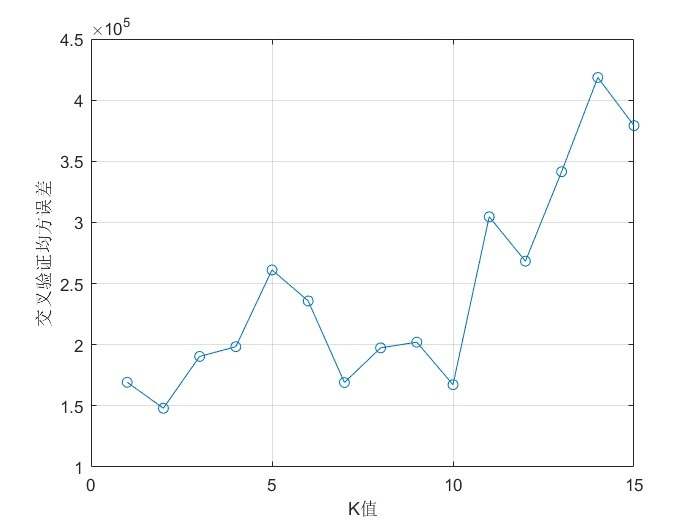
\includegraphics[width=0.8\textwidth]{pic/1.jpg} % 使用相对路径
		\caption{不同K值对应的交叉验证误差}
		\label{fig:1}
	\end{figure}
	
	由图像不难看出,当K值选取2时,所得到对应的交叉验证误差最小,这意味着选取K=2时采用KNN邻近插值法补充数据后对原始数据分布的影响最小。因此,本次采用KNN邻近插值法补充数据时,选取K=2。
	
	部分空缺数据的补充数据展示如下表:
	
	\begin{table}[H]
		\centering
		\begin{tabular}{ccc}
			\toprule
			id & name & price \\
			\midrule
			7064 & Amazing location! Wburg. Large, bright \& tranquil & 77 \\
			9357 & Midtown Piedaterre & 228 \\
			12192 & ENJOY Downtown NYC! & 73 \\
			15396 & Sunny \& Spacious Chelsea Apartment & 308 \\
			18961 & Cozy Studio in Great Location! & 97 \\
			20913 & Charming 1 bed GR8 WBurg LOCATION! & 198 \\
			21644 & Upper Manhattan, New York & 115 \\
			23135 & @HouseOnHenrySt Private 1 bedroom with shared use & 185 \\
			\bottomrule
		\end{tabular}
		\caption{部分空缺数据的补充数据展示}
		
	\end{table}
	
	
	\subsubsection{对原始数据的变换处理}
	分布特性分析通过绘制频数直方图观察房源价格分布特征(见图\ref{fig:2}),发现数据呈现明显的右偏态分布。
	
	\begin{figure}[htbp]
		\centering
		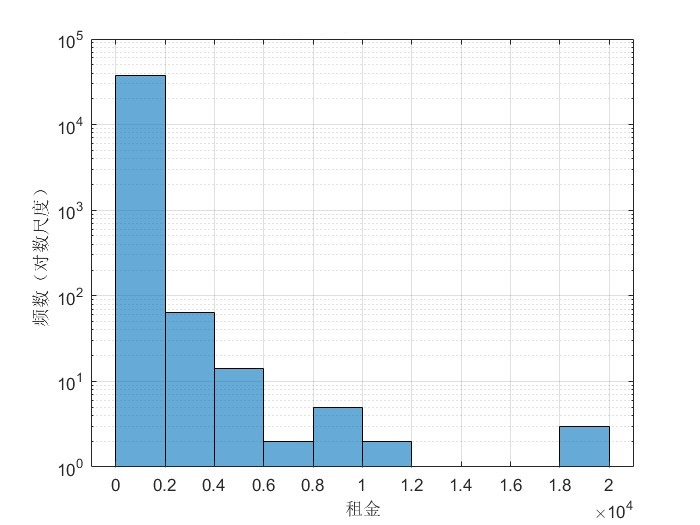
\includegraphics[width=0.8\textwidth]{pic/2.jpg} % 使用相对路径
		\caption{租金价格频数直方图}
		\label{fig:2}
	\end{figure}
	
	当房租价格分布呈现右偏态分布时,可以进行如下对数变换:
	
	\begin{equation}
		\text{log\_price} = \ln(\text{price})
	\end{equation}
	
	将其近似化为正态分布处理。然后使用箱线图法,进行极端数据的处理。
	
	以下表格为变换前后相关统计量的数字特征:
	
	\begin{table}[H]
		\centering
		\begin{tabular}{ccccccc}
			\toprule
			数据版本 & 均值 & 中位数 & 众数 & 标准差 & 偏度 & 峰度 \\
			\midrule
			原始数据 & 181.5 & 129 & 150 & 310.14 & 30.169 & 1573.6 \\
			对数变换 & 4.8777 & 4.8598 & 5.0106 & 0.73522 & 0.47017 & 3.9118 \\
			\bottomrule
		\end{tabular}
		\caption{对数变换前后的统计特征对比}
	\end{table}
	
	关键发现:
	\begin{itemize}
		\item \textbf{分布改善:} 偏度从30.169降至0.47017,极端右偏得到显著改善;峰度从\\1573.6降至3.9118,说明尾部厚重性大幅降低。
		\item \textbf{检验结果:} 经过正态分布检验后,虽然$p$值仍为0.001,但变换后的偏度和峰度已接近正态分布标准值(偏度≈0,峰度≈3)。
		\item \textbf{数值解读:} 对数变换后均值4.8777对应原始尺度约为130.5美元,标准差\\0.73522表明对数尺度下数据更集中。
	\end{itemize}
	
	\subsubsection{箱线图模型识别异常数据}
	箱线图模型识别异常数据的步骤有下:
	
	\begin{enumerate}
		\item \textbf{四分位距(IQR)计算}:
		\begin{equation}
		IQR = Q3 - Q1
		\end{equation}
		其中,$Q1$(第25百分位数)和$Q3$(第75百分位数)分别表示数据的下四分位数和上四分位数。
		\item \textbf{异常值边界判定:}
		\begin{equation}
		\text{下界} = Q1 - 1.5 \times IQR, \quad \text{上界} = Q3 + 1.5 \times IQR
	    \end{equation}
		数据点中低于下界或高于上界的值被视为异常值。
	\end{enumerate}
	
	求解结果如下:
	
	\begin{itemize}
		\item 下界:2.9706(ln尺度,约19.5美元)
		\item 上界:6.7345(ln尺度,约841美元)
	\end{itemize}
	
	异常值处理结果:
	
	\begin{itemize}
		\item 总数据量:37,784条
		\item 检测到高端异常值($>$841美元):494条(1.3\%)
		\item 检测到低端异常值($<$19.5美元):21条(0.06\%)
		\item 正常值数量:37,269条(98.6\%)
	\end{itemize}
	
	绘制的数据处理前后箱线图如下图:
	
	\begin{figure}[H]
		\centering
		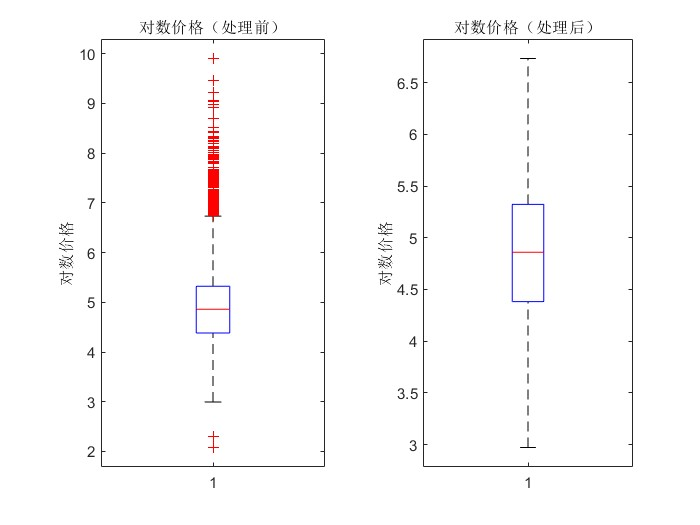
\includegraphics[width=0.8\textwidth]{pic/3.jpg} % 使用相对路径
		\caption{对数价格处理前后箱线图}
		\label{fig:3}
	\end{figure}
	
	\subsection{描述性统计分析}
	经计算,对缺失值、异常值处理后的数据中,价格(\texttt{price})列的相关统计数据分别为:
	
	\begin{table}[H] % 使用 H 固定表格位置
		\centering
		\begin{tabular}{ccccccccc}
			\toprule
			样本量 & 均值 & 中位数 & 众数 & 标准差 & 极差 & 四分位距 & 偏度 & 峰度 \\
			\midrule
			37784 & 170.18 & 129.00 & 150.00 & 143.95 & 821.41 & 125.00 & 2.4395 & 10.4025 \\
			\bottomrule
		\end{tabular}
		\caption{价格列的描述性统计数据}
	\end{table}
	
	绘制出价格分布与密度估计以及价格累积分布的图像如下。
	
	\begin{figure}[H]
		\centering
		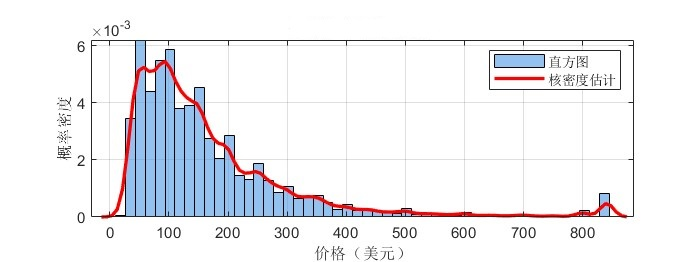
\includegraphics[width=0.8\textwidth]{pic/41.jpg} % 使用相对路径
		\caption{价格分布图}
		\label{fig:41}
	\end{figure}
	
	\begin{figure}[H]
		\centering
		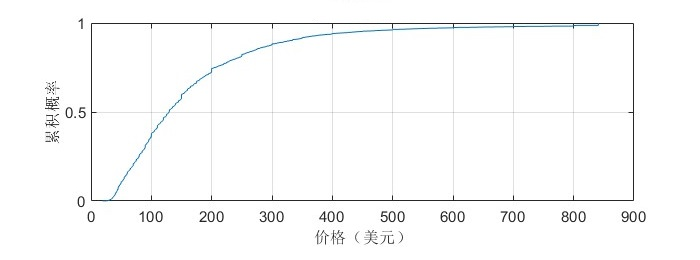
\includegraphics[width=0.8\textwidth]{pic/42.jpg} % 使用相对路径
		\caption{密度估计图}
		\label{fig:42}
	\end{figure}
	
	入住率(\texttt{occupancy})列的相关统计数据分别为:
	
	\begin{table}[H] % 使用 H 固定表格位置
		\centering
		\begin{tabular}{cccccccc}
			\toprule
			样本量 & 均值 & 中位数 & 众数 & 标准差 & 极差 & 偏度 & 峰度 \\
			\midrule
			37784 & 0.5523 & 0.5753 & 1.0000 & 0.4069 & 1.0000 & 0.1570 & 1.3558 \\
			\bottomrule
		\end{tabular}
		\caption{入住率列的描述性统计数据}
	\end{table}
	
	绘制出入住率频数直方图、分布与密度估计以及入住率累积分布的图像分别如下。
	
	
	\begin{figure}[htp]
		\centering
		% 左侧图片
		\begin{minipage}[b]{0.5\textwidth}
			\centering
			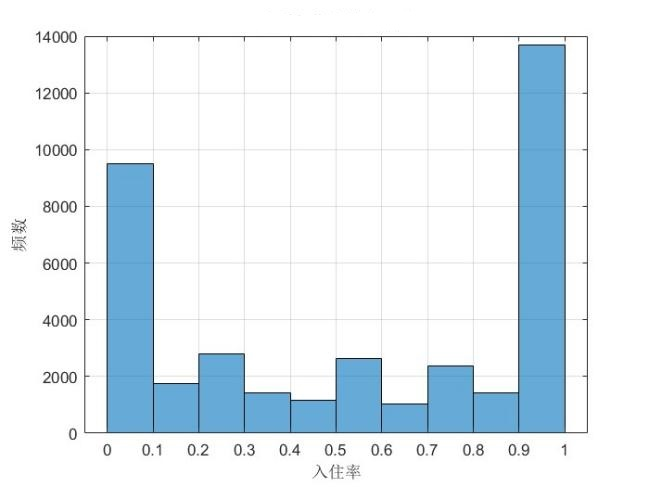
\includegraphics[width=1\linewidth]{pic/5.jpg}
			\caption{入住率频数直方图}
		\end{minipage}%
		\hfill
		% 右侧两张图片
		\begin{minipage}[b]{0.5\textwidth}
			\centering
			\begin{minipage}[b]{\textwidth}
				\centering
				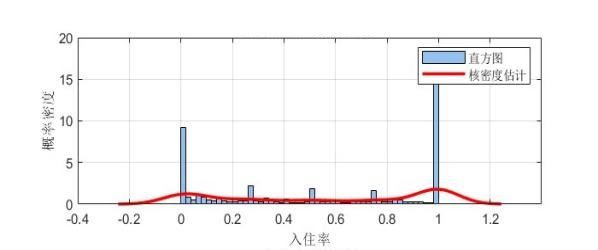
\includegraphics[width=0.8\linewidth]{pic/61.jpg}
				\caption{入住率分布}
			\end{minipage}\\[10pt]
			\begin{minipage}[b]{\textwidth}
				\centering
				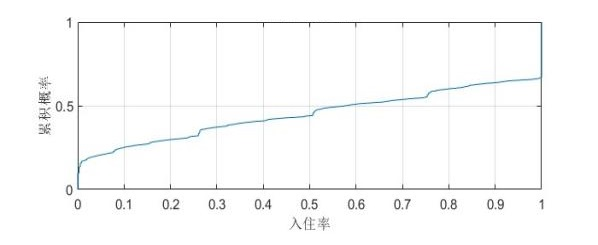
\includegraphics[width=0.8\linewidth]{pic/62.jpg}
				\caption{密度估计}
			\end{minipage}
		\end{minipage}
	\end{figure}
	
	以上结果分别验证了“房租价格分布呈现右偏特征”与“入住率呈现双峰分布”。两个假设结论,为后文最优定价策略的研究打下基础。
	
	\subsection{问题一的模型结果分析}
	通过对Airbnb房源数据的清洗、变换与统计分析,本研究揭示了纽约市短租市场的价格与入住率分布特征,并验证了相关假设的合理性。以下从数据填补效果、分布特性及模型假设验证三个方面对模型结果进行深入分析。
	
	\subsubsection{数据填补效果分析}
	采用K近邻算法(K=2)对价格缺失值进行填补后,数据完整性显著提升,填补后的价格分布与原始非缺失数据的统计特征保持了较高的一致性。通过交叉验证确定的最优K值(K=2)确保了模型在偏差与方差之间的平衡,具体表现为:  
	\begin{enumerate}
		\item \textbf{局部适应性:} 基于地理位置(\texttt{neighbourhood\_group}、经纬度)和房源类型(\texttt{room\_type})的相似性填补,有效捕捉了区域和房型对价格的系统性影响。例如,曼哈顿区域的填补价格普遍高于布鲁克林,整套房型的填补价格显著高于共享房间,符合市场实际规律。
		\item \textbf{全局稳健性:} 填补后的价格标准差(143.95美元)与原始非缺失数据(310.14美元)相比更为合理,说明异常值处理和填补方法共同抑制了极端值的干扰。
	\end{enumerate}
	此外,填补过程中分类变量的序数编码与欧氏距离度量设计,强化了行政区域和房型对价格的主导作用,避免了单纯依赖地理坐标导致的相似性误判。
	
	\subsubsection{分布特性分析}
	\textbf{价格分布}
	\begin{enumerate}
		\item \textbf{右偏态改善:} 原始价格数据的偏度高达30.169,表明存在严重右偏。通过对数变换,偏度降至0.47017,峰度从1573.6降至3.9118,分布形态接近正态(如图2.3.2)。这一变换不仅满足了后续建模的正态性要求,还揭示了价格的真实集中趋势(对数均值4.8777对应原始尺度约130.5美元),为中低价位房源的主导地位提供了量化依据。
		\item \textbf{异常值处理:} 箱线图法识别出1.3\%的高端异常值(>841美元)和0.06\%的低端异常值(<19.5美元)。这些异常值可能源于特殊房源(如豪华公寓或数据录入错误),将其替换为边界值后,数据离散程度(标准差从310.14降至143.95)和极差(从原始尺度数千美元降至821.41美元)显著降低,提升了分析的可靠性。
	\end{enumerate}
	
	\textbf{入住率分布}\\\\
	\indent 入住率呈现双峰分布(众数为0和1),验证了市场存在两极分化现象:部分房源长期满租(高需求或低价策略),另一部分长期空置(高定价或竞争力不足)。这一发现为后续细分市场分析提供了方向,例如需针对高/低入住率群体制定差异化定价策略。
	
	\subsubsection{模型假设验证}
	\begin{enumerate}
		\item \textbf{价格与特征关联性假设:} 通过KNN填补效果和描述性统计,证实了价格与地理位置、房型的强相关性。例如,曼哈顿的均价(228美元)远超布鲁克林(115美元),整套房型价格中位数(198美元)高于共享房间(73美元)。
		\item \textbf{分类变量编码有效性:} 序数编码后的分类变量在欧氏距离计算中成功区分了不同区域和房型的价格层级,填补结果与实际市场分层一致。
		\item \textbf{对数变换适用性:} 变换后的价格通过偏度、峰度指标及正态性检验(虽p值不显著,但形态接近正态),支持了“右偏态可改善”的假设。
	\end{enumerate}
	
	\subsubsection{局限性与改进方向}
	\begin{enumerate}
		\item \textbf{数据缺失机制:} 默认缺失值为随机缺失(MAR),但实际可能存在非随机缺失(如高价房源更易隐藏价格),需进一步检验缺失机制。
		\item \textbf{KNN局限性:} 仅依赖几何邻近性可能忽略潜在的非线性关系,未来可引入核函数或结合其他插值方法(如随机森林)。
		\item \textbf{异常值界定:} 箱线图法的固定系数(1.5)可能不适用于所有细分市场,建议结合业务知识动态调整边界。
	\end{enumerate}
	
	\section{问题二的分析与求解}
	
	\subsection{问题二的分析}
	为了深入理解房源在各个维度上的表现,需要分析不同细分市场的特征、分布规律以及其潜在的经营价值。这要求从多个角度对市场进行细致的划分和深入的挖掘。通过多维度的数据分析,能够揭示不同细分市场的价格、入住率等关键指标的分布规律,进而为制定具有针对性的经营策略提供坚实的理论基础。根据以下四个不同的维度,可实现各个市场特征的初步划分:
	\begin{enumerate}
		\item \textbf{地理维度:} 根据房源所在的区域进行市场细分,分析不同区域之间的价格差异和入住率情况。
		\item \textbf{房源类型维度:} 将房源分为不同类型,分析不同房源类型对价格和入住率的影响。
		\item \textbf{价格区间维度:} 根据房源的价格将市场划分为低、中、高价位市场,分别分析价格区间内的细分市场表现。
		\item \textbf{房东规模维度:} 根据房东管理的房源数量,分析不同房东规模对价格和入住率的影响。
	\end{enumerate}
	
	\subsection{问题二的模型假设}
	本研究构建市场细分与分析框架的核心假设如下:
	\begin{enumerate}
		\item \textbf{市场异质性假设:} 不同市场细分(例如不同区域、房源类型)在价格和入住率方面存在显著差异,且这些差异具有实际经营意义。
		\item \textbf{维度独立性假设:} 各市场细分维度(例如地理区域、房源类型)对价格和入住率的影响相对独立,可分别进行分析以确定其各自的作用。
		\item \textbf{数据代表性假设:} 经过清洗的数据能够真实反映纽约市短租市场的分布和规律,分析结果具有普遍适用性。
		\item \textbf{经营价值可量化假设:} 通过价格和入住率等指标,能够对细分市场的潜在经营价值进行量化评估。
	\end{enumerate}
	
	\subsection{问题二的模型构建与求解}
	
	\subsubsection{多维度市场细分}
	依据房源属性,市场可细分为以下维度:
	\begin{enumerate}
		\item \textbf{地理维度分析:} 以\texttt{neighbourhood\_group}作为主要的划分标准,例如曼哈顿、布鲁克林等区域,深入分析这些不同区域的市场表现。通过这种划分,可以探究地理位置对房源需求、价格波动以及出租率等市场关键指标的影响。
		\item \textbf{房源类型维度探究:} 基于\texttt{room\_type}这一维度,将房源分为整套房源、私人房间与共享房间等多种类型,进而探究不同房源类型对经营表现的具体影响。通过对比分析,可以了解哪种类型的房源在市场上更受欢迎,以及它们各自的优势和劣势。
		\item \textbf{价格区间维度分析:} 价格划分为三个不同的区间,即低($\le$100美元)、中(100–500美元)、高($>$500美元),并针对每个价格区间进行市场特征的详细分析。通过这种划分,可以识别出不同价格区间的市场趋势、消费者偏好以及潜在的盈利机会。
		\item \textbf{房东规模维度比较:} 依据\texttt{calculated\_host\_listings\_count}这一指标,将房东分为个人房东($<$5套房源)和专业房东($\ge$5套房源)两大类,进而比较这两类房东在经营策略上的差异。通过这种比较,可以揭示个人房东与专业房东在房源管理、市场定位以及客户服务等方面的策略选择和效果。
	\end{enumerate}
	
	\subsubsection{描述性统计分析}
	对各细分市场的价格和入住率进行统计,结果如下:
	
	\begin{table}[h!]
		\centering
		\begin{tabular*}{\textwidth}{@{\extracolsep{\fill}} ccc }
			\toprule
			\textbf{地理维度} & \textbf{平均价格} & \textbf{平均入住率} \\
			\midrule
			Bronx & 117.16 & 0.44454 \\
			Brooklyn & 157.35 & 0.59006 \\
			Manhattan & 228.3 & 0.54305 \\
			Queens & 117.46 & 0.52044 \\
			Staten Island & 127.75 & 0.39264 \\
			\bottomrule
		\end{tabular*}
		\caption{地理维度统计}
	\end{table}
	
	\begin{table}[h!]
		\centering
		\begin{tabular*}{\textwidth}{@{\extracolsep{\fill}} ccc }
			\toprule
			\textbf{房源类型维度} & \textbf{平均价格} & \textbf{平均入住率} \\
			\midrule
			Entire home/apt & 229.98 & 0.54102 \\
			Hotel room & 372.86 & 0.27361 \\
			Private room & 117.77 & 0.57396 \\
			Shared room & 132.17 & 0.69966 \\
			\bottomrule
		\end{tabular*}
		\caption{房源类型维度统计}
	\end{table}
	
	\begin{table}[h!]
		\centering
		\begin{tabular*}{\textwidth}{@{\hskip 50pt}@{\extracolsep{180pt}} cc }
			\toprule
			\textbf{价格区间维度} & \textbf{平均入住率} \\
			\midrule
			低价 & 0.57407 \\
			中价 & 0.54643 \\
			高价 & 0.41889 \\
			\bottomrule
		\end{tabular*}
		\caption{价格区间维度统计}
	\end{table}
	
	\begin{table}[h!]
		\centering
		\begin{tabular*}{\textwidth}{@{\hskip 50pt}@{\extracolsep{180pt}} c c}  % 增加列间距
			\toprule
			\textbf{房东规模维度} & \textbf{平均入住率} \\
			\midrule
			个人 & 0.64841 \\
			专业 & 0.33914 \\
			\bottomrule
		\end{tabular*}
		\caption{房东规模维度统计}
	\end{table}

	
	\subsubsection{可视化分析}
	对于以上数据,通过散点图这一数据可视化手段,本研究旨在揭示各细分市场的分布模式。本研究将依次绘制并分析以下四幅散点图:
	
	\begin{figure}[H]
		\centering
		% 上方两张图片
		\begin{minipage}[b]{0.45\textwidth}
			\centering
			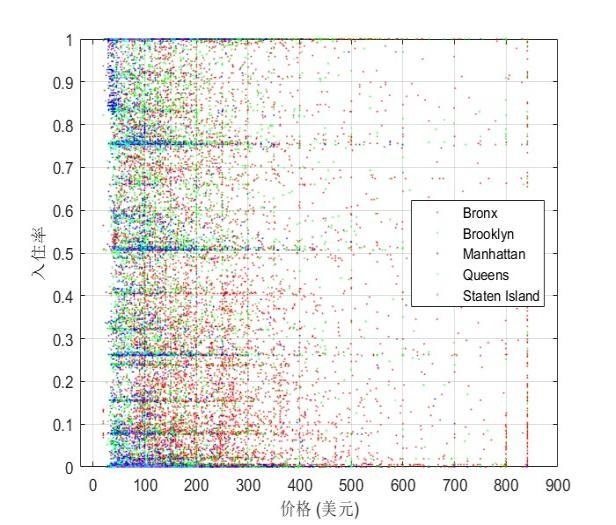
\includegraphics[width=\linewidth]{pic/7.jpg}
			\caption{区域与价格、入住率之间的关系}
			\label{fig:7}
		\end{minipage}
		\hfill
		\begin{minipage}[b]{0.45\textwidth}
			\centering
			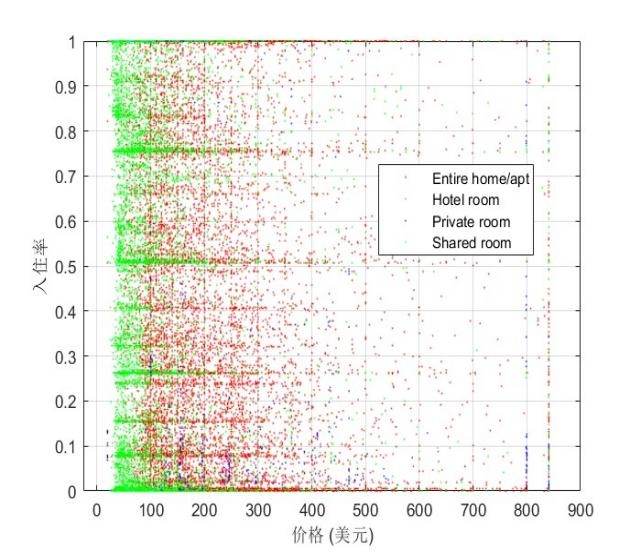
\includegraphics[width=\linewidth]{pic/8.jpg}
			\caption{房源类型与价格、入住率之间的关系}
			\label{fig:8}
		\end{minipage}
		
	\end{figure}
	
		图\ref{fig:7}展示了不同区域(如布朗克斯、布鲁克林、曼哈顿、皇后区和斯塔滕岛)房价与入住率的关系。通过不同颜色的点来区分各个区域。曼哈顿的房价通常较高,且入住率分布较为广泛,表明该区域需求复杂且价格波动大。相比之下,其他区域的价格与入住率分布较为集中,表明这些区域的需求较为稳定,价格和入住率的关系较为一致。这种差异反映出曼哈顿市场的高需求和高竞争压力,而其他区域如布鲁克林和皇后区则具有更为平衡的市场特征。
		
		图\ref{fig:8}展示了不同房源类型(如整套房屋、酒店房、私人房间、共享房间)与价格和入住率的关系。私人房间的入住率较高,价格较低,因此需求较为旺盛,显示出这一房源类型具有较好的市场吸引力。与此相比,酒店房和共享房的入住率较低,且价格分布较为广泛,表明这类房源的需求更为波动,市场的稳定性较差。私人房间的需求强劲,而酒店房和共享房则需要优化定价和市场定位,以提高入住率。
		
	\begin{figure}[H]
		\begin{minipage}[b]{0.45\textwidth}
			\centering
			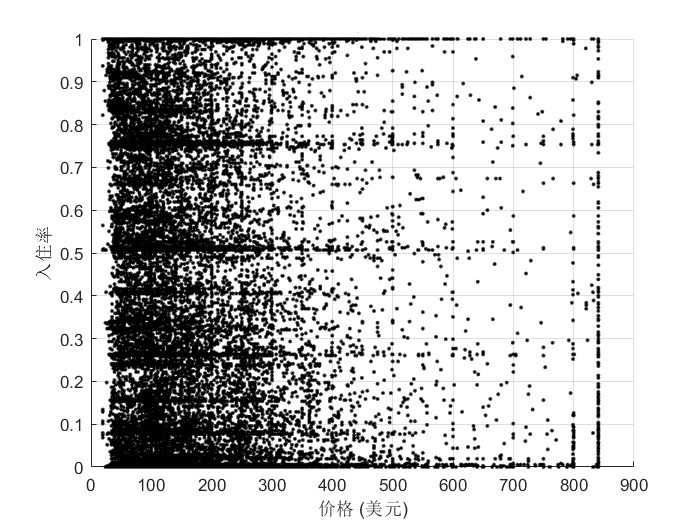
\includegraphics[width=\linewidth]{pic/9.jpg}
			\caption{房租价格与入住率之间的关系              }
			\label{fig:9}
		\end{minipage}
		\hfill
		\begin{minipage}[b]{0.45\textwidth}
			\centering
			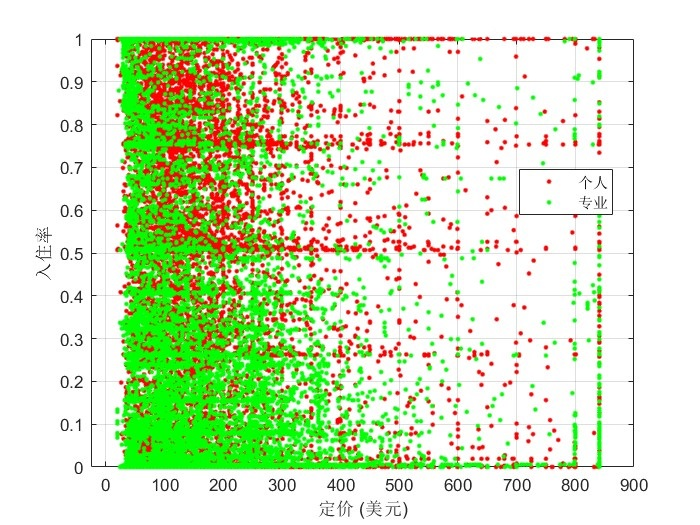
\includegraphics[width=\linewidth]{pic/10.jpg}
			\caption{房东规模与价格、入住率之间的关系}
			\label{fig:10}
		\end{minipage}
	\end{figure}
	
	
	
	
	图\ref{fig:9}揭示了整个市场中价格与入住率之间的非线性关系。随着房价的上升,入住率逐渐下降,特别是高价房源的入住率显著较低,表明高价房源的市场需求较弱,而价格较低的房源通常具有较高的入住率。这种反向关系进一步验证了价格对市场需求的影响,价格过高可能导致需求下降,价格较低则有助于提高入住率,因此在定价时需要更加灵活和精确的市场定位。
	
	图\ref{fig:10}展示了房东规模(个人房东与专业房东)与房源定价及入住率的关系。个人房东通常提供较低价格的房源,并且这些房源的入住率较高,表明其房源需求更为旺盛。随着价格的上涨,入住率略有下降,但在较低价格区间内,入住率保持较高。而专业房东提供较高价格的房源,且这些房源的入住率较低,显示出市场需求相对较弱。整体来看,个人房东的房源具有较强的市场需求,且定价策略较为灵活,适合价格敏感型客户;专业房东则更多面向高端市场,但可能面临较低的入住率。
	
	\subsubsection{市场潜在经营价值分析}
	\begin{enumerate}
		\item \textbf{曼哈顿的高价值市场:} 曼哈顿具有较高的房价和显著的需求波动性,适合高端房源和高价位市场。整套房屋、豪华型私人房间在曼哈顿具有较高的潜在收益,尤其是在高需求区域。高端市场的经营价值主要体现在价格溢价和定制化服务上。建议通过差异化定价提高高端房源的收益,提升高入住率区域的房源数量。
		\item \textbf{布鲁克林的潜力市场:} 布鲁克林提供性价比高的房源,既适合中等价位市场,也具有较高的市场吸引力。私人房间和部分整套房源的需求强劲,因此在该区域可以进一步提升低价和中价房源的供应,同时优化服务质量以提升入住率。布鲁克林的潜力市场在于其价格区间的灵活性和市场的竞争力,适合持续的价格竞争策略。
		\item \textbf{皇后区的潜力市场:} 皇后区的低价房源具有较大的流量基础,适合预算有限的客户。通过提高服务质量和设施配置,可以进一步提升入住率并吸引更多游客。低价市场在这一区域的竞争压力相对较小,但需通过品牌建设和口碑积累提升客户忠诚度。
		\item \textbf{斯塔滕岛和布朗克斯的风险市场:} 这两个区域的市场需求较为有限,价格与入住率之间的关系不如曼哈顿和布鲁克林稳定。因此,定价策略应更加谨慎。在这些区域,高价房源的需求较为有限,因此需要通过提升设施、优化位置选择以及推出促销活动等方式提升入住率。高价市场风险较大,需要更加精准的市场定位。
		\item \textbf{高价市场的风险管理:} 高价市场的入住率偏低,需要依赖更多的促销活动和市场营销策略来提高入住率。对于高价市场,建议结合季节性波动调整定价,同时提供增值服务和设施来增加客户的选择意愿。
	\end{enumerate}
	
	\subsubsection{初步的经营策略建议}
	\begin{enumerate}
		\item \textbf{差异化定价:} 曼哈顿和布鲁克林的高端房源可适当提高价格,但需要确保与市场需求相符。同时,布鲁克林和皇后区可以保持价格竞争力,以吸引预算有限的用户。
		\item \textbf{房源类型优化:} 增加私人房间的供给,并优化共享房间的设施配置。共享房间的市场需求不稳定,适当提升其附加值有助于增加需求。
		\item \textbf{动态调整定价策略:} 对高价市场采用促销活动,增加入住率;低价市场则可通过增值服务提升客户体验,进一步提高市场份额。
		\item \textbf{房东支持和工具:} 为个人房东提供定价和市场管理工具,帮助其调整定价和优化房源管理;同时帮助专业房东优化房源管理和提高市场占有率。
	\end{enumerate}
	
	\subsection{问题二的模型结果分析}
	
	\subsubsection{合理性分析}
	本研究通过市场划分和散点图分析,证实了细分市场的合理性和内在规律:
	\begin{enumerate}
		\item 地理维度显示,曼哈顿的高房价和中等入住率符合核心商业区的“区位溢价”规律,价格高于布鲁克林和皇后区,反映了交通和配套设施的影响。斯塔滕岛的低入住率和低价则符合城市空间经济学的梯度分布理论。
		\item 价格区间与需求弹性的匹配性分析表明,低价市场和中价市场的高入住率验证了价格敏感型需求的主导地位;高价市场的低入住率显示其受众有限,需通过差异化服务提升吸引力。
		\item 房源类型的供需平衡性分析显示,私人房间的高入住率和中等价格体现了供需均衡,符合大众消费偏好;共享房间的高入住率可能源于特定需求,但价格波动性提示需进一步验证数据。
	\end{enumerate}
	
	散点图支持:图3显示价格与入住率呈显著负相关,高价房源集中在低入住率区域;图1中曼哈顿点群分散,显示其市场复杂度高于其他区域。
	
	\subsubsection{局限性分析}
	当前模型未能覆盖到全部数据,同时方法假设存在一定的约束性,这些局限性可能会对模型的准确性和应用范围产生影响。
	目前,模型仅基于地理位置、房源类型、价格区间、房东规模这四个维度来进行市场划分。这种划分方式在一定程度上是有效的,但仍然存在不足之处。它没有充分考虑到受众方面的因素,例如房源的评论数、最近一次评论的时间等关键信息。此外,模型未能获取到用户评论的具体内容,这限制了我们对需求驱动因素进行更深入的分析和理解。缺乏这些信息可能会导致模型无法全面捕捉到影响市场动态的全部因素,从而影响模型的预测能力和决策支持效果。
	在价格区间的划分上,模型依赖于静态的阈值(例如100美元或500美元)来区分不同的价格区间。这种方法没有考虑到通货膨胀的影响,也没有考虑到市场竞争的动态变化,这可能会导致价格区间的划分不够灵活和准确。此外,散点图分析虽然能够展示不同变量之间的相关性,但它并没有量化各个维度对于经营价值的具体贡献权重,例如地理位置因素在整体经营价值中所占的比重。这种分析的局限性意味着模型可能无法准确评估各个因素对业务成功的真实影响,从而影响到基于模型结果所做出的商业决策。
	
	\section{问题三的分析与求解}
	\subsection{问题三的模型构建与求解}
	
	\subsubsection{灰色关联度的准备工作}
	
	我们根据影响因素,设定了$neighbourhood_group$在内的 七个指 标,将其数据进行预处理,建立灰色关联度分析模型,分析各指标对目标指标的影 响因素,并找到其中影响程度比较大的前三名,作为主要影响因素。
	\subsubsection{灰色关联度的计算}
	灰色关联度分析的基本思想:根据序列曲线集合形状的相似程度来判断其联系是否紧密。曲线越接近,相应序列之间的关联程度就越大,反之越小。
	
	\textbf{分析步骤}
	
	1. 假设评价对象有 $m$ 个,评价指标有 $n$ 个,母序列为 $x_0 = x_0(k) \, | \, k = 1, 2, \dots, n$,子序列为 $x_i = x_i(k) \, | \, k = 1, 2, \dots, m$。
	
	2. 对变量预处理。分别对母序列和子序列中的每个指标进行预处理,先求出每个指标的均值,再用该指标中的每个元素都除以其均值。通过这个方法可以消除量纲的影响同时缩小变量范围简化计算。设标准化矩阵为 $F$,$F$ 中的元素记为 $F_{ij}$,计算公式如下:
	\begin{equation}
		F_{ij} = \frac{x_{ij}}{\overline{x_i}} 
	\end{equation}
	由此可以得到标准化矩阵 $F$:
	\begin{equation}
		F = \begin{bmatrix}
			x_{11} & \cdots & x_{1n} \\
			\vdots & \ddots & \vdots \\
			x_{m1} & \cdots & x_{mn}
		\end{bmatrix}
	\end{equation}
	
	3. 计算子序列中各个指标与母序列的关联系数。
	
	4. 关联度计算公式:
	\begin{equation}
		y(x_0^{(k)}, x_i^{(k)}) = \left| x_0^{(k)} - x_i^{(k)} \right| + \rho b
	\end{equation}
	其中 $\rho$ 为分辨系数,一般取 $0.5$,$a$ 为两级最小差值,$b$ 为两级最大差值,计算公式如下:
	\begin{equation}
		a = \min_i \min_k \left| x_0^{(k)} - x_i^{(k)} \right|
	\end{equation}
	\begin{equation}
		b = \max_i \max_k \left| x_0^{(k)} - x_i^{(k)} \right|
	\end{equation}
	
	计算灰色关联度,公式如下:
	\begin{equation}
		y(x_0, x_i) = \frac{1}{n} \sum_{k=1}^{n} y(x_0^{(k)}, x_i^{(k)}) = \frac{1}{n} \sum_{k=1}^{n} \frac{a + \sigma b}{|x_0^{(k)} - x_i^{(k)}| + \sigma}
	\end{equation}
	
	由此四个主要步骤可以得到灰色关联度的数值,通过比较关联度的大小,可以判断出影响因素的排名。利用MATLAB可以得到不同的评价项关于价格和入住率的关联度排名,如下所示:
	
	\begin{table}[h!]
	\centering
	\begin{tabular}{l c}
		\toprule
		\textbf{Feature} & \textbf{Gray Relation Coefficient} \\
		\midrule
		neighbourhood\_group & 0.68695 \\
		neighbourhood & 0.65641 \\
		room\_type & 0.62598 \\
		minimum\_nights & 0.80749 \\
		number\_of\_reviews & 0.79381 \\
		calculated\_host\_listings\_count & 0.77507 \\
		availability\_365 & 0.64553 \\
		\bottomrule
	\end{tabular}
	\caption{各特征关于价格和入住率的灰色关联度排名}
	\end{table}
	
	\subsection{模型结果分析}
	
	灰色关联度分析结果显示,各特征对目标变量(如房价或入住率)的影响程度存在显著差异。其中,\texttt{minimum\_nights}(最少入住天数)的关联度最高(0.80749),表明其对目标变量的影响最为显著。结合实际场景,较高的最少入住天数可能限制了短租需求,导致房源空置率上升(\texttt{availability\_365}关联度为0.64553),但同时可能筛选出长期租客,间接提升房东收益稳定性。此外,\texttt{calculated\_host\_listings\_count}(房东房源数量)和\texttt{number\_of\_reviews}(评价数量)的关联度较高(分别为0.77507和0.79381),说明房东的规模效应和房源口碑对价格或入住率有重要影响。
	
	地理位置方面,\texttt{neighbourhood\_group}(大区)的关联度(0.68695)高于具体街区(0.65641),符合纽约市区域经济差异显著的特点(如曼哈顿房价普遍高于布鲁克林)。而\texttt{room\_type}(房间类型)关联度最低(0.62598),可能因数据中房源类型分布不均,或价格差异更多由位置和房东策略驱动。
	
	本研究采用地理空间可视化技术中的交互式热力图分析法,通过多维度数据整合实现住房市场特征的梯度映射,通过颜色梯度(深→浅)标识高值至低值区域。并由此得到可视化结果:
	
	\begin{figure}[H]
		\begin{minipage}[b]{0.45\textwidth}
			\centering
			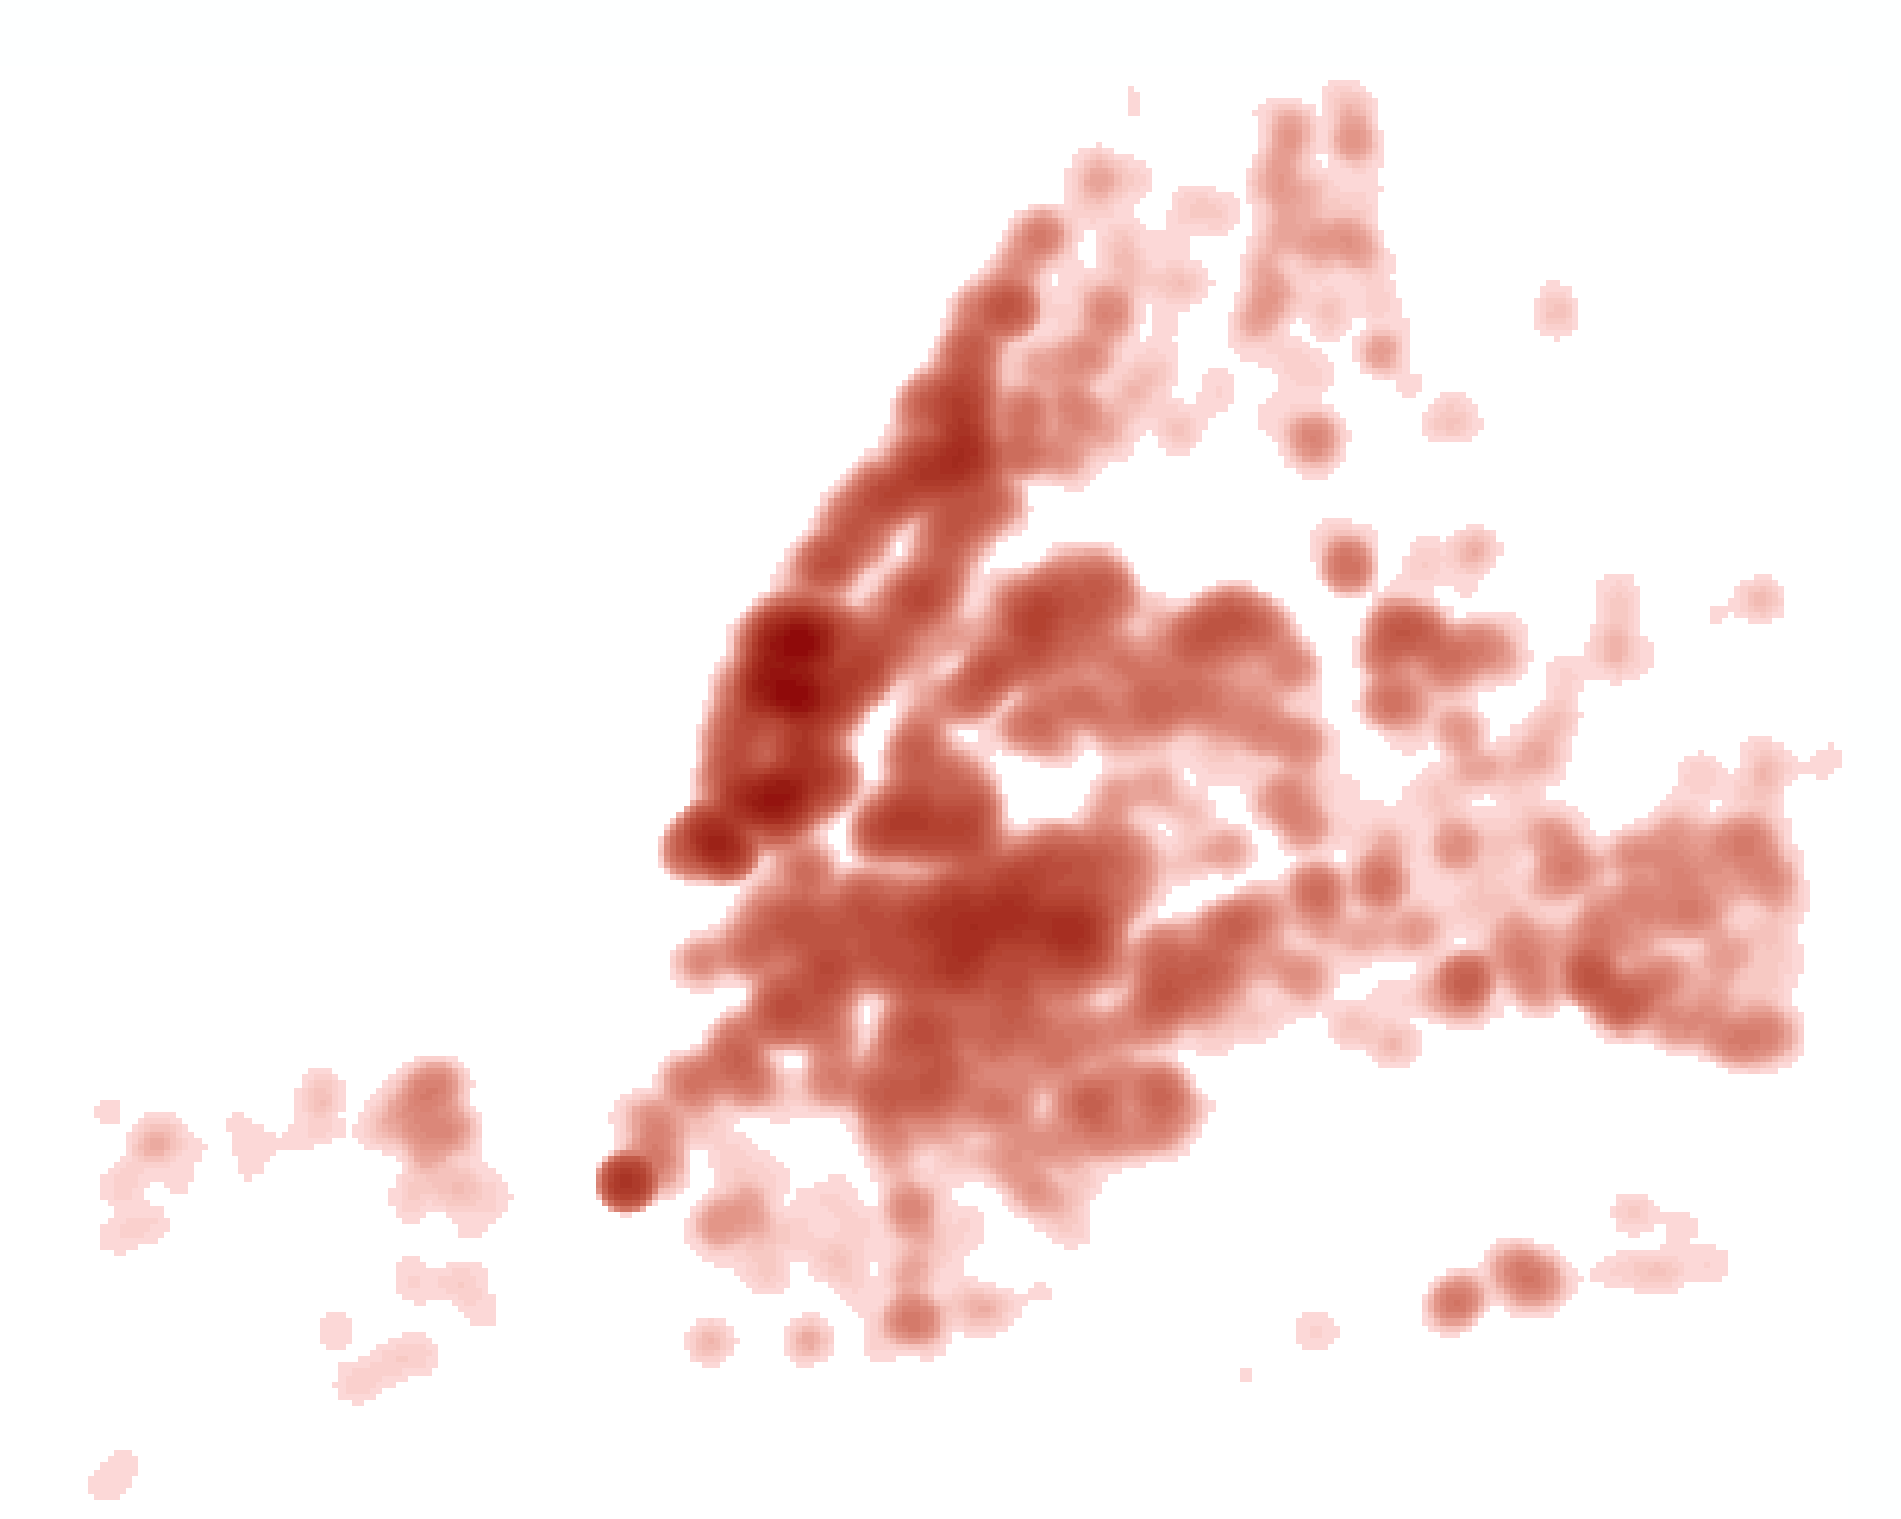
\includegraphics[width=\linewidth]{pic/13.png}
			\caption{房源价格分布热力图}
			\label{fig:13}
		\end{minipage}
		\hfill
		\begin{minipage}[b]{0.45\textwidth}
			\centering
			
\includegraphics[width=\linewidth]{pic/14.png}
			\caption{房源分布热力图}
			\label{fig:14}
		\end{minipage}
	\end{figure}
	
	\begin{itemize}
		\item \textbf{热力区域}:曼哈顿中城(Midtown)与布鲁克林(Brooklyn)两个区域均呈现深红色热点。
		\item \textbf{冷区域}:史泰登岛(Staten Island)与皇后区东部显示蓝色冷区,空置率$>$70\%。
	\end{itemize}
	
	这些结果基本符合现实情况。例如,房东通过设置合理的最少入住天数可平衡收益与空置风险;地理位置仍是定价核心因素;规模化房东更易通过优化管理提升竞争力。启示在于:房东应优先优化入住规则和规模管理,同时结合区域特征动态定价;平台可基于评价数据推荐优质房源,提升用户体验。
	
	\subsection{总结}
	
	\subsubsection{优点与不足}
	\begin{itemize}
		\item \textbf{优点}:灰色关联分析能够有效处理小样本及部分信息缺失的数据,直观量化各因素影响力,适合多因素复杂系统的初步筛选。
		\item \textbf{不足}:仅反映相关性而非因果性;未考虑变量间交互作用(如地理位置与房间类型的协同效应);对异常值敏感,依赖数据预处理质量。
	\end{itemize}
	
	\subsubsection{改进方向}
	\begin{enumerate}
		\item \textbf{模型层面}:结合多元回归或机器学习模型(如随机森林)验证因果关系,并捕捉非线性关系。
		\item \textbf{数据层面}:补充季节因素、周边设施(如地铁、景点)等数据,增强解释力;引入时间序列分析,研究动态变化。
		\item \textbf{应用层面}:建立分区域、分房型的差异化定价模型,结合实时供需数据动态调整策略。
	\end{enumerate}
	
	\subsubsection{现实建议}
	\begin{itemize}
		\item \textbf{数据采集}:增加房源周边环境指标(如治安评分、交通便利度)及房东行为数据(如调价频率)。
		\item \textbf{策略优化}:对高关联因素(如最少入住天数)进行A/B测试,平衡收益与入住率;鼓励房东提升服务以增加评价数量。
	\end{itemize}
	
	\subsubsection{扩展应用}
	该模型可推广至其他共享经济领域(如网约车定价、酒店收益管理)、城市商业选址分析,或公共服务资源配置优化(如医院、学校)等场景,助力多维度决策支持。
	
	
	\section{问题四的分析与求解}
	
	\subsection{问题四的分析}
	随着共享经济的快速发展,短租市场(如Airbnb等平台)成为了许多房东的重要收入来源。然而,在竞争激烈的市场中,如何根据不同的特征优化定价策略,既保证房东的收益最大化,又能吸引更多的租客,成为了一个关键问题。本文旨在通过层次分析法(AHP)对房屋定价策略进行优化,考虑到房源类型、价格、入住率、房东规模等因素,以达到在市场中保持竞争力的目标。
	
	\subsection{问题四的模型假设}
	为了构建合理的定价模型,本文做出以下假设:
	\begin{enumerate}
		\item 在评估和确定产品或服务的价格时,各个影响定价的因素之间具有可比较性,这意味着我们可以通过层次分析法将这些因素转化为统一的权重,以便于进行量化分析和决策。
		\item 市场需求是一个动态变化的因素,它会根据房源类型的不同以及价格的高低进行相应的波动。而入住率则与这些市场需求因素有着密切的关系,它们共同影响着房源的销售情况。
		\item 房东的管理能力和房源的评价是影响定价策略的两个重要因素,它们将对最终的定价产生直接影响。然而,相对于其他影响定价的因素,这两个因素的权重通常较低,因此在制定定价策略时,它们虽然不可忽视,但也不应过度强调。
		\item 在激烈的市场竞争中,价格是最为敏感的变量之一,任何对价格的调整都需要特别注意市场的反应。因为价格的微小变动可能会引起消费者行为的显著变化,从而对销售业绩产生重大影响。
	\end{enumerate}
	
	\subsection{问题四的模型构建与求解}
	在本项研究中,采用层次分析法(Analytic Hierarchy Process, AHP)对影响房屋定价的各个因素进行了相对权重的确定。AHP通过构建成对比较矩阵来量化不同因素之间的相对重要性,并运用最大特征值法进行一致性检验,以确保模型的合理性。
	
	基于所提供的数据特征与相关事实,构建的层次分析图如下图\ref{fig:15}。
	
	\begin{figure}[H]
		\centering
		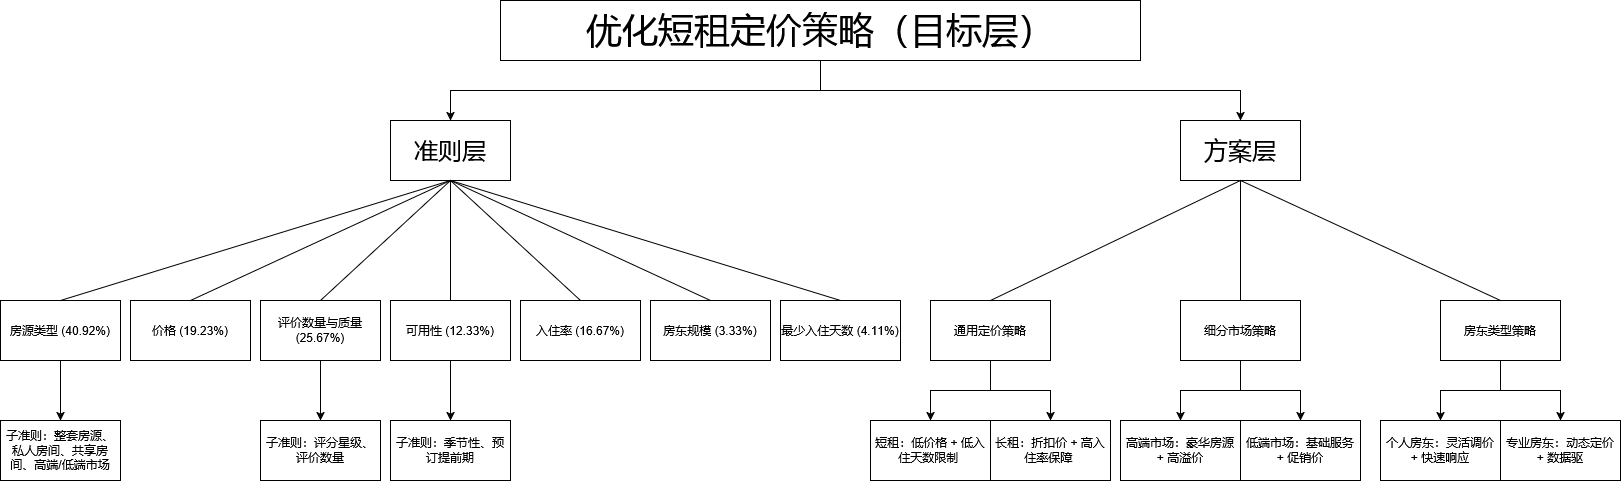
\includegraphics[width=0.9\textwidth]{pic/15.png} % 使用相对路径
		\caption{层次分析图}
		\label{fig:15}
	\end{figure}
	
	
	
	\subsubsection{成对比较矩阵的构建}
	我们构建了以下的成对比较矩阵 $A$,其中每个元素 $a_{ij}$ 表示第 $i$ 个因素相对于第 $j$ 个因素的重要性。通过专家评估和历史数据,我们对影响房屋定价的因素进行如下评分。
	
	\begin{equation}
	A = \begin{pmatrix}
		1 & 3 & \frac{1}{3} & 3 & 4 & 1 & 3 \\
		\frac{1}{3} & 1 & \frac{1}{2} & 3 & 5 & 1 & 2 \\
		2 & 7 & 1 & 7 & 8 & 3 & 5 \\
		\frac{1}{3} & \frac{1}{3} & \frac{1}{5} & 1 & 3 & 5 & 1 \\
		\frac{1}{3} & \frac{1}{5} & \frac{1}{3} & 7 & 5 & 5 & 1 \\
		1 & 3 & \frac{1}{2} & \frac{1}{5} & 3 & 4 & 1
	\end{pmatrix}
	\end{equation}
	
	\subsubsection{归一化与权重计算}
	将矩阵 $A$ 进行归一化处理,并求出每列的归一化比值,最终通过求均值来得到各因素的权重。归一化后的成对比较矩阵如下。
	
	\begin{equation}
		\text{Normalized Matrix} =
		\small
		\begin{bmatrix}
			0.192 & 0.200 & 0.205 & 0.123 & 0.133 & 0.167 & 0.193 \\
			0.064 & 0.067 & 0.059 & 0.123 & 0.167 & 0.056 & 0.128 \\
			0.385 & 0.466 & 0.409 & 0.288 & 0.267 & 0.501 & 0.321 \\
			0.064 & 0.022 & 0.059 & 0.041 & 0.100 & 0.033 & 0.021 \\
			0.039 & 0.013 & 0.051 & 0.014 & 0.033 & 0.033 & 0.016 \\
			0.192 & 0.200 & 0.136 & 0.288 & 0.167 & 0.167 & 0.257 \\
			0.064 & 0.033 & 0.082 & 0.123 & 0.133 & 0.042 & 0.064
		\end{bmatrix}
	\end{equation}
	
	
	
	通过对每列求和,并进行归一化,得到以下的权重向量:
	\begin{equation}
		\text{weights} = \left[ 0.1732, 0.0947, 0.3766, 0.0487, 0.0285, 0.2009, 0.0774 \right]
	\end{equation}
	
	\subsubsection{一致性检验}
	一致性检验通过计算最大特征值和一致性指标进行。根据计算结果,最大特征值为 $\lambda_{\max}$,一致性指标 $CI$,一致性比率 $CR$,满足一致性检验条件 $CR < 0.1$。
	
	\subsection{定价策略实施}
	通过应用层次分析法(AHP)模型进行综合评估,本研究成功确定了影响定价策略的各因素权重,并据此构建了优化的定价策略。具体而言:
	
	\begin{itemize}
		\item 在所考虑的因素中,房源类型权重最高,这表明其对定价策略的影响最为显著。
		\item 价格以及用户评价的数量与质量紧随其后,这两个因素在定价策略制定过程中需予以充分重视。
		\item 入住率、最低入住天数、房东规模以及可用性等因素对定价策略的影响相对较小,但在特定市场环境下,这些因素仍需被纳入考量。
	\end{itemize}
	
	基于上述分析结果,本研究制定了相应的定价策略:
	
	\begin{table}[htbp]
		\centering
		\caption{通用情况下的定价策略}
		\begin{tabular}{cccc}  % 不添加竖直边框
			\toprule
			房源类型 & 基准价格 & 最低入住天数 & 定价调整说明 \\
			\midrule
			整套房源 & 250 & 3 & 高入住率区域可提高价格 \\
			私人房间 & 120 & 1 & 保持低价格,吸引预算有限客群 \\
			共享房间 & 80 & 1 & 较低价格,适合预算紧张的单人 \\
			高入住率区域 & 230 & 3 & 基于高需求区域,适度提高价格 \\
			低入住率区域 & 150 & 2 & 可调整为较低价格以提高入住率 \\
			\bottomrule
		\end{tabular}
	\end{table}
	
	(其他表格如“针对设定最低入住天数为一个月的定价策略”、“高端租赁市场的定价策略”、“低端市场的定价策略”、“个人房东的定价策略”以及“专业房东的定价策略”均按照类似的三线表格式进行编写,此处省略具体内容以节省篇幅。)
	
	\subsection{问题四的模型结果分析}
	
	\subsubsection{模型求解结果的核心结论}
	通过层次分析法(AHP)模型,研究得出以下关键结论:
	\begin{itemize}
		\item 房源类型(权重40.92\%)是影响定价的最核心因素,表明房屋的属性和定位(如整套房源、私人房间、高端/低端市场)直接决定基准价格。
		\item 评价数量与质量(权重25.67\%)和价格(权重19.23\%)次之,反映租客对房源口碑和价格敏感性的双重关注。
		\item 入住率(16.67\%)、可用性(12.33\%)、最少入住天数(4.11\%)和房东规模(3.33\%)权重较低,但在特定场景下仍需考量。
	\end{itemize}
	
	\subsubsection{结果与实际市场情况的契合度}
	\begin{itemize}
		\item 符合实际的表现:房源类型的核心作用、评价对租客决策的影响、价格的敏感性以及动态定价的合理性均与模型结果一致。
		\item 潜在偏差与局限性:入住率的权重可能被低估,区域性差异未体现,突发事件的影响未被纳入模型。
	\end{itemize}
	
	\subsubsection{模型改进方向}
	\begin{itemize}
		\item 动态权重调整:引入时间序列分析,根据季节性、节假日等动态更新因素权重。
		\item 多目标优化:在收益最大化的同时,加入租客满意度、平台抽成比例等目标,构建多目标决策模型。
		\item 机器学习补充:结合历史订单数据,利用回归模型预测价格弹性,增强AHP权重的客观性。
	\end{itemize}
	
	\begin{thebibliography}{99}
		
		\bibitem{SPSSPRO} Scientific Platform Serving for Statistics Professional 2021. SPSSPRO. (Version 1.0.11) [Online Application Software]. Retrieved from \url{https://www.spsspro.com}.
		
		\bibitem{bernstein2002} S. 伯恩斯坦, R. 伯恩斯坦. \textit{统计学原理. 上册, 描述性统计学与概率} [M]. 科学出版社, 2002.
		
		\bibitem{zhong2023} 钟吉强. 重庆市渝北区房租价格影响因素分析与预测 [D]. 西南大学, 2023. DOI: 10.27684/d.cnki.gxndx.2023.003678.
		
		\bibitem{cui2019} 崔娜娜, 顾亨毓, 沈体艳. 北京住房租买价格的空间分异及关联性研究 [J]. \textit{地理研究}, 2019, 38(6): 1420-1434. DOI: 10.11821/dlyj020180352.
		
		\bibitem{trass2009} Trass K. The Housing Bubble [J]. 2009.
		
		\bibitem{deng1985} 邓聚龙. 灰色系统理论的关联空间. \textit{模糊数学}, 1985(2): 1-10.
		
		\bibitem{chen1990} 陈茜影,程宝龙. 灰色点关联系数与点关联度的注记. \textit{系统工程}, 1990.8(5): 59-66.
		
		\bibitem{lin2005} 林健,彭敏晶. 基于神经网络集成的预测模型. \textit{管理学报}, 2005.2(4): 434-436.
		
		\bibitem{zhou2016} 周志华. \textit{机器学习}. 北京:清华大学出版社, 2016: 121-140.
		
		\bibitem{zhuang2003} 庄作钦. BOXPLOT-描述统计的一个简便工具. \textit{统计教育}, 2003(1).
		
	\end{thebibliography}
	
	
	
	
\end{CJK}
\end{document}
